
\tikzstyle{process} = [rectangle, minimum width=3cm, minimum height=1cm, text centered, draw=black]
\tikzstyle{arrow} = [thick,->,>=stealth]

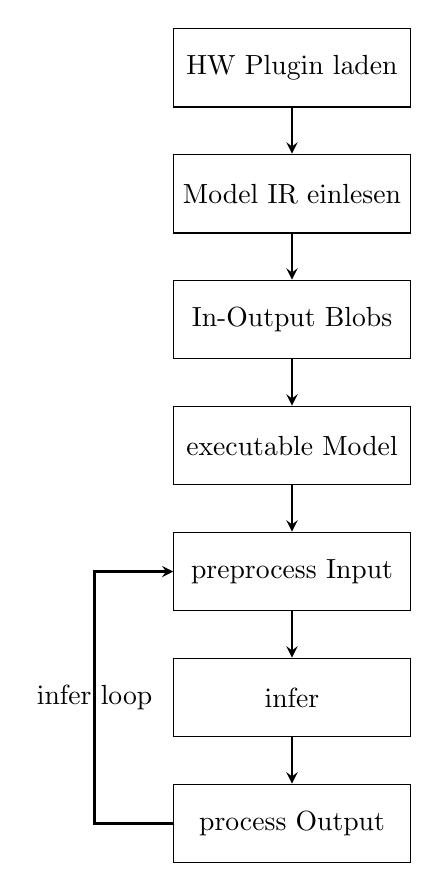
\begin{tikzpicture}[node distance=1.6cm]
    \node (hw)      [process]                   {HW Plugin laden};
    \node (ir)      [process, below of=hw]      {Model IR einlesen};
    \node (io)      [process, below of=ir]      {In-Output Blobs};
    \node (execNet) [process, below of=io]      {executable Model};
    \node (prepIn)  [process, below of=execNet] {preprocess Input};
    \node (infer)   [process, below of=prepIn]  {infer};
    \node (procOut) [process, below of=infer]   {process Output};

    \draw [arrow] (hw) -- (ir);
    \draw [arrow] (ir) -- (io);
    \draw [arrow] (io) -- (execNet);
    \draw [arrow] (execNet) -- (prepIn);
    \draw [arrow] (prepIn) -- (infer);
    \draw [arrow] (infer) --  (procOut);

    \draw [arrow] (procOut.west) -- +(-1,0) |- node[pos=0.25] {infer loop} (prepIn);

    
\end{tikzpicture}
